% ============================== CHAPTER 3 ===================================
\chapter{Requirement Engineering}
\label{ch:requirements}

Requirement engineering for \setu{} is complicated by the fact that the system
has two distinct execution environments with almost nothing in common. Training
runs once per direction on a datacentre GPU with tens of gigabytes of memory and
unrestricted network access; inference runs repeatedly on a phone or an ARM
board with no network at all. A requirement that is trivial in one environment
may be impossible in the other. This chapter therefore specifies the two
environments separately, models the system conceptually through the standard
object-oriented and structured views, and states the requirements independently
of how they are satisfied.

\section{Software and Hardware Tools Used}
\label{sec:tools}

\subsection{Hardware Requirements}
\label{subsec:hw}

Table~\ref{tab:hwtrain} gives the training hardware. The primary training
platform was an NVIDIA A40-16Q --- a 16\,GB vGPU slice of a 48\,GB A40, software
partitioned rather than MIG partitioned --- on a Debian host. A local CPU-only
workstation was used for development, testing and the pipeline's smaller runs;
its constraints are listed because they shaped several design decisions that
survive into the final system.

\begin{table}[H]
\centering
\caption{Hardware used for training and development}
\label{tab:hwtrain}
\begin{tabular}{@{}p{3.1cm} p{5.2cm} p{5.6cm}@{}}
\toprule
\rowcolor{headblue}
\textbf{Component} & \textbf{Training platform (GPU VM)} & \textbf{Development platform (local)} \\
\midrule
Processor        & Host CPU, Debian & 8-core x86-64 \\
\rowcolor{rowgrey}
Accelerator      & NVIDIA A40-16Q, 16\,GB vGPU slice, Ampere cc 8.6, driver 535, CUDA 12.2 & None (CPU only) \\
System memory    & Sufficient to hold teacher and student concurrently & 7.4\,GB \\
\rowcolor{rowgrey}
Storage          & $\approx$640\,GB, 575\,GB free & Standard SSD \\
Purpose          & Teacher distillation, student training, quantisation, evaluation & Pipeline development, unit and integration testing, small-scale runs \\
\bottomrule
\end{tabular}
\end{table}

The 7.4\,GB ceiling on the development machine is worth recording, because it
produced a real design constraint rather than a mere inconvenience. A
52-million-parameter student with an AdamW optimiser state and batch-64
activations exceeded available memory, drove the machine into 5.6\,GB of swap
and slowed training to roughly four seconds per step. The response --- a smaller
development student and a batch size of 16 --- is why the repository carries two
parallel configuration sets, \texttt{model.yaml}/\texttt{training.yaml} for CPU
development and \texttt{model.gpu.yaml}/\texttt{training.gpu.yaml} for GPU
training.

Table~\ref{tab:hwdeploy} gives the deployment target. The constraint that
matters is that inference must complete within 500\,ms on a CPU with no
accelerator, using an artifact no larger than 200\,MB.

\begin{table}[H]
\centering
\caption{Target deployment hardware}
\label{tab:hwdeploy}
\begin{tabular}{@{}p{3.6cm} p{10.3cm}@{}}
\toprule
\rowcolor{headblue}
\textbf{Requirement} & \textbf{Specification} \\
\midrule
Processor   & ARM Cortex-A55 class or better; commodity x86-64 CPU also supported \\
\rowcolor{rowgrey}
Accelerator & None. Inference uses the ONNX Runtime CPU execution provider exclusively \\
Memory      & Approximately 512\,MB of working memory per loaded direction \\
\rowcolor{rowgrey}
Storage     & 104\,MB per translation direction, plus roughly 2\,MB for the SentencePiece tokenizer \\
Network     & Required only for the initial one-time model download; not used thereafter \\
\bottomrule
\end{tabular}
\end{table}

\subsection{Software Tools Used}
\label{subsec:sw}

\begin{longtable}{@{}p{2.7cm} p{4.4cm} p{6.8cm}@{}}
\caption{Software stack, by pipeline stage}
\label{tab:swstack}\\
\toprule
\rowcolor{headblue}
\textbf{Stage} & \textbf{Tool / library} & \textbf{Role in the system} \\
\midrule
\endfirsthead
\multicolumn{3}{c}{\textit{Table \thetable{} --- continued from previous page}}\\
\toprule
\rowcolor{headblue}
\textbf{Stage} & \textbf{Tool / library} & \textbf{Role in the system} \\
\midrule
\endhead
\midrule
\multicolumn{3}{r}{\textit{continued on next page}}\\
\endfoot
\bottomrule
\endlastfoot

Language     & Python 3.11 / 3.12 & Implementation language for the entire pipeline. Python 3.14 was abandoned because the teacher's rotary remote modelling code requires \texttt{transformers} below 4.54 \\
\rowcolor{rowgrey}
Data         & Hugging Face \texttt{datasets} & Streaming ingestion of the Samanantar corpus \\
Teacher      & \texttt{transformers} ($\geq$4.42, $<$4.54), \texttt{IndicTransToolkit}, \texttt{einops}, \texttt{sentencepiece} & Loads and runs the IndicTrans2 distilled-200M teacher; \texttt{IndicProcessor} handles script normalisation and entity placeholders \\
\rowcolor{rowgrey}
Training     & PyTorch $\geq$2.6 (CUDA 12.4), \texttt{torchvision} 0.21 & Student training. Torch 2.6 is a hard floor: the CVE-2025-32434 guard in newer \texttt{transformers} refuses to \texttt{torch.load} the teacher's non-safetensors weights on older versions \\
Tokenizer    & SentencePiece & 16{,}000-token unigram vocabulary trained per direction, with 23 FLORES language tags reserved so token identifiers stay stable as languages are added \\
\rowcolor{rowgrey}
Quantisation & \texttt{optimum}, ONNX, ONNX Runtime & FP32 ONNX export, ORT validation, progressive INT8 and INT4 quantisation \\
Inference    & ONNX Runtime (CPU provider) & Executes the quantised student on device \\
\rowcolor{rowgrey}
Evaluation   & \texttt{sacrebleu}, COMET (optional) & BLEU and chrF with reproducible signatures; COMET for languages where n-gram overlap understates quality \\
API          & FastAPI, Uvicorn, Pydantic & REST service with typed request and response models \\
\rowcolor{rowgrey}
Frontend     & Next.js (App Router), TypeScript, React & Browser client and offline progressive web application \\
Testing      & \texttt{pytest} & 85 automated tests across all modules \\
\rowcolor{rowgrey}
Tooling      & Git, tmux, Conda/venv & Version control; tmux keeps multi-hour training alive across SSH disconnections \\
OS           & Debian (training), Ubuntu 22.04 LTS, Android 11+ (deployment) & \\
\end{longtable}

\subsubsection{Environment Constraints Discovered During Development}

Four environment problems were encountered in sequence on the training VM, each
diagnosed and then encoded into the runner script so that a clean run never
repeats them. They are recorded here because they are requirements in practice,
even though no specification predicted them.

\begin{enumerate}[leftmargin=0.75in]
  \item \textbf{Transformers versus Torch (CVE-2025-32434).} The VM shipped
        \texttt{transformers} 4.36; the installation floor raised it to 4.53,
        whose \texttt{torch.load} security guard refuses the teacher's
        non-safetensors \texttt{.bin} weights unless Torch is 2.6 or newer.
        Resolution: upgrade to Torch 2.6.0+cu124, which works on driver 535
        through CUDA minor-version compatibility.
  \item \textbf{Torchvision ABI mismatch.} After the Torch upgrade, loading the
        teacher failed with \texttt{operator torchvision::nms does not exist},
        because \texttt{torchvision} 0.20.1 was built against Torch 2.5.1.
        Resolution: \texttt{torchvision} 0.21.0 (cu124).
  \item \textbf{vGPU allocator crash.} Training died on its first CUDA
        allocation with \texttt{CUDA driver error: operation not supported}. The
        cause was \texttt{PYTORCH\_CUDA\_ALLOC\_CONF=expandable\_segments:True},
        whose CUDA virtual-memory APIs are unsupported on an A40-16Q vGPU slice.
        Resolution: the flag now defaults to \texttt{False}.
  \item \textbf{Resume re-clone bug.} The runner's clone check looked for
        \texttt{.git} inside the \texttt{SETU/} subdirectory, but Git places it
        at the clone root, so every resume attempted to re-clone over an existing
        tree that already held the expensive distilled corpus. Resolution: detect
        the repository by the root \texttt{.git} or \texttt{pyproject.toml}.
\end{enumerate}

\subsubsection{Dataset and Model Access Constraints}

The \texttt{ai4bharat/BPCC} dataset and all official \texttt{ai4bharat/%
indictrans2-*} checkpoints are access-gated on Hugging Face and return HTTP 401
without an authenticated account that has accepted the terms. The project
therefore uses the ungated \texttt{prajdabre/rotary-indictrans2-\{indic-en,%
en-indic\}-dist-200M} teachers and the ungated Samanantar corpus. No ungated
Indic-to-Indic teacher exists at all, which is the direct cause of the
English-pivot design in Section~\ref{subsec:mod5}.

\section{Conceptual / Analysis Modelling}
\label{sec:modelling}

This section models \setu{} from two complementary perspectives. The
object-oriented view --- use case, sequence, activity, state chart and class
diagrams --- describes actors, interactions and structure. The structured view
--- data flow and entity-relationship diagrams --- describes how data moves and
how it is related. Together they define what the system does before
Chapter~\ref{ch:design} decides how it does it.

A property visible in every model below is that \setu{} has two disjoint
lifecycles. The \emph{offline training lifecycle} is executed by an ML engineer,
once per direction, and consumes a GPU. The \emph{online inference lifecycle} is
executed by an end user, repeatedly, on a device. An end user never touches a
training component, and the training components are absent from the deployed
artifact entirely.

\subsection{Use Case Diagram}
\label{subsec:usecase}

Three actors interact with the system. The \textbf{End User} translates text.
The \textbf{ML Engineer} runs the training pipeline. The \textbf{Edge Device} is
a secondary actor that hosts the quantised model and executes inference.

\begin{figure}[H]
\centering
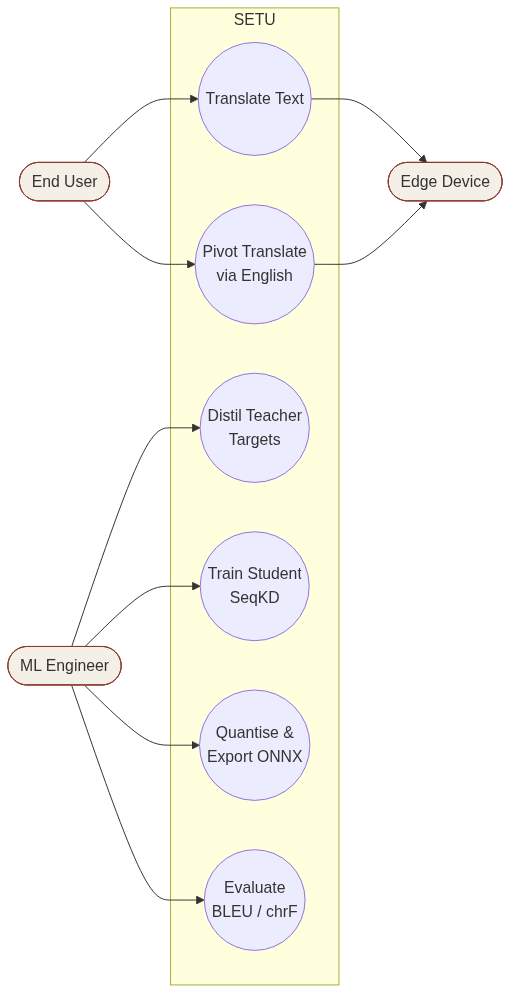
\includegraphics[width=0.94\textwidth, height=0.72\textheight, keepaspectratio]{figures/use_case.png}
\caption{Use case diagram --- End User, ML Engineer and Edge Device actors}
\label{fig:usecase}
\end{figure}

\begin{table}[H]
\centering
\caption{Use case specifications}
\label{tab:usecases}
\begin{tabular}{@{}L{2.7cm} L{1.9cm} L{4.3cm} L{4.6cm}@{}}
\toprule
\rowcolor{headblue}
\textbf{Use case} & \textbf{Actor} & \textbf{Precondition} & \textbf{Postcondition} \\
\midrule
Translate Text & End User & A trained model exists for the requested direction & Translated text returned with measured latency \\
\rowcolor{rowgrey}
Pivot Translate & End User & No direct model exists, but both source\arrowto{}English and English\arrowto{}target models exist & Translated text returned, flagged \texttt{pivot="en"} \\
List Languages & End User & Language registry loaded & 22 scheduled languages plus English returned, trained ones marked \\
\rowcolor{rowgrey}
Distil Teacher Targets & ML Engineer & Cleaned corpus available; teacher checkpoint reachable & Distilled corpus of teacher one-best targets written \\
Train Student & ML Engineer & Distilled corpus available; GPU available & Trained checkpoint plus a training report written \\
\rowcolor{rowgrey}
Quantise \& Export & ML Engineer & Trained checkpoint exists & INT8 and INT4 ONNX artifacts with a quantisation report \\
Evaluate & ML Engineer & Student and teacher both available & BLEU, chrF and student/teacher ratio recorded \\
\rowcolor{rowgrey}
Execute Inference & Edge Device & Quantised model and tokenizer present locally & Translation produced with zero network calls \\
\bottomrule
\end{tabular}
\end{table}

\subsection{Sequence Diagram}
\label{subsec:sequence}

Figure~\ref{fig:sequence} traces a single translation request. The significant
branch is the pivot: when a directly trained model exists the engine performs
one hop, and when it does not --- every Indic-to-Indic pair --- the engine
performs two, passing the intermediate English string from the first student to
the second. The response carries the summed latency of both hops and a
\texttt{pivot} field so that the caller can tell the two cases apart.

\begin{figure}[H]
\centering
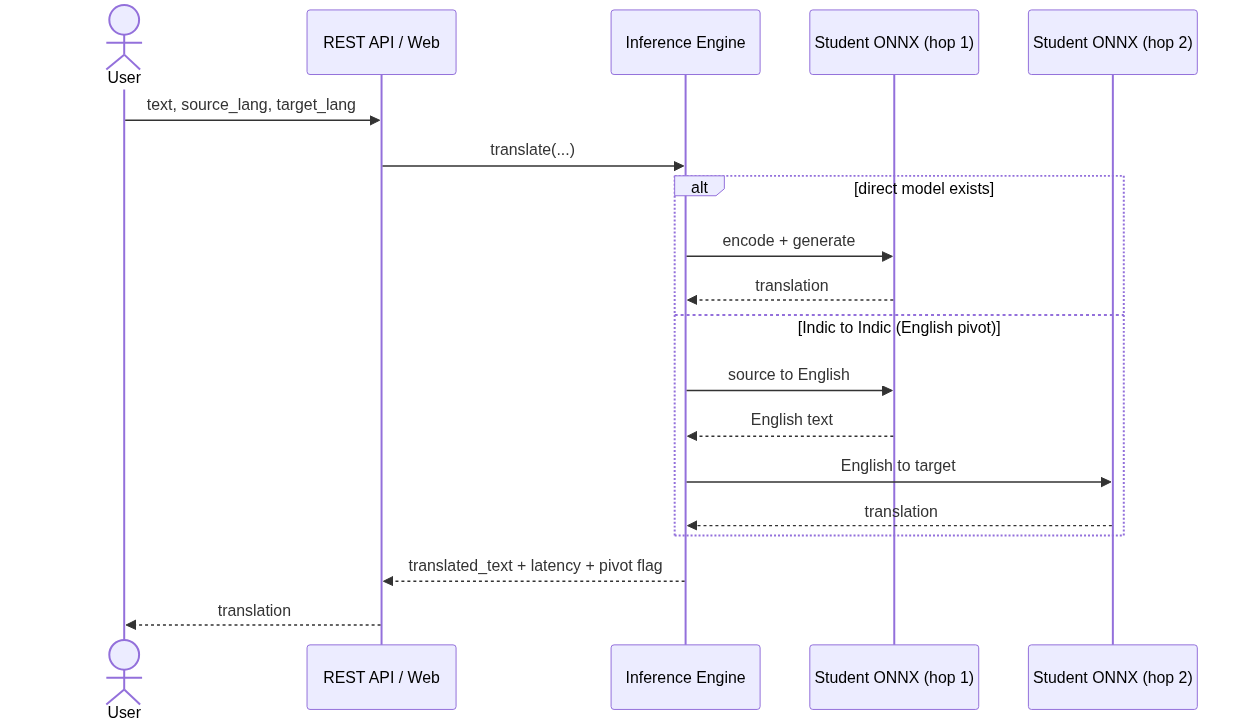
\includegraphics[width=0.96\textwidth, height=0.72\textheight, keepaspectratio]{figures/sequence.png}
\caption{Sequence diagram --- direct translation and the two-hop English pivot}
\label{fig:sequence}
\end{figure}

\subsection{Activity Diagram}
\label{subsec:activity}

Figure~\ref{fig:activity} shows the full training and deployment activity flow.
Everything above the dividing line executes once per direction on a GPU;
everything below executes on the user's device. The two decision points are the
quality gate --- does the student reach 80\,\% of teacher BLEU --- and the
routing decision at inference time.

\begin{figure}[H]
\centering
\scalebox{0.84}{%
\begin{tikzpicture}[node distance=6.5mm and 9mm]
  \node[circle, fill=black, minimum size=3.4mm, inner sep=0] (start) {};
  \node[proc, below=of start, minimum width=46mm] (load)  {Load Samanantar corpus (streamed)};
  \node[proc, below=of load, minimum width=46mm]  (clean) {Normalise scripts, filter by length,\\ratio and script, remove duplicates};
  \node[proc, below=of clean, minimum width=46mm] (teach) {Teacher decodes one-best target\\for every source sentence};
  \node[proc, below=of teach, minimum width=46mm] (train) {Train 52.6\,M student\\(PAD-masked cross-entropy, warmup,\\label smoothing, gradient clipping)};
  \node[proc, below=of train, minimum width=46mm] (eval)  {Evaluate BLEU / chrF against\\held-out human references};
  \node[dec,  below=6mm of eval, text width=24mm] (gate)  {ratio\\$\geq 0.80$?};
  \node[proc, right=16mm of gate, minimum width=32mm, fill=red!6] (retune) {Lower learning rate\\to $3\times10^{-4}$,\\add data, retrain};
  \node[proc, below=8mm of gate, minimum width=46mm] (quant) {Export ONNX, quantise INT8 then INT4\\(411\,MB $\rightarrow$ 103.9\,MB)};
  \node[proc, below=of quant, minimum width=46mm] (ship)  {Package model + tokenizer,\\deploy to device};

  \draw[fl] (start) -- (load);
  \draw[fl] (load)  -- (clean);
  \draw[fl] (clean) -- (teach);
  \draw[fl] (teach) -- (train);
  \draw[fl] (train) -- (eval);
  \draw[fl] (eval)  -- (gate);
  \draw[fl] (gate)  -- node[lbl,above]{no} (retune);
  \draw[fl] (retune.north) |- ([yshift=3mm]train.north) -- (train.north);
  \draw[fl] (gate)  -- node[lbl,right]{yes} (quant);
  \draw[fl] (quant) -- (ship);

  \draw[dashed, black!50] ([xshift=-14mm,yshift=-5mm]ship.west) -- ([xshift=30mm,yshift=-5mm]ship.east)
        node[pos=0.06, below, font=\scriptsize\itshape, black!60, anchor=north west]
        {offline training $\uparrow$ \quad on-device inference $\downarrow$};

  \node[proc, below=13mm of ship, minimum width=46mm] (req)  {Receive text, source and target language};
  \node[dec,  below=6mm of req, text width=26mm] (direct) {direct model\\available?};
  \node[proc, right=14mm of direct, minimum width=32mm] (pivot) {Hop 1: source $\rightarrow$ English\\Hop 2: English $\rightarrow$ target};
  \node[proc, below=8mm of direct, minimum width=46mm] (single) {Single-hop inference};
  \node[proc, below=of single, minimum width=46mm] (out) {Return translation, latency, pivot flag};
  \node[circle, draw=black, thick, minimum size=4mm, inner sep=0, below=6mm of out] (endo) {};
  \node[circle, fill=black, minimum size=2.4mm, inner sep=0] at (endo) {};

  \draw[fl] (ship) -- (req);
  \draw[fl] (req)  -- (direct);
  \draw[fl] (direct) -- node[lbl,above]{no} (pivot);
  \draw[fl] (direct) -- node[lbl,right]{yes} (single);
  \draw[fl] (pivot.south) |- (out.east);
  \draw[fl] (single) -- (out);
  \draw[fl] (out) -- (endo);
\end{tikzpicture}}
\caption{Activity diagram --- offline training pipeline (above) and on-device inference (below)}
\label{fig:activity}
\end{figure}

\subsection{State Chart Diagram}
\label{subsec:statechart}

A model in \setu{} passes through a well-defined sequence of states.
Figure~\ref{fig:statechart} records them, including the two transitions that
were exercised in practice: the collapse detected at evaluation and the recovery
achieved by retraining at a lower learning rate on the same distilled corpus.

\begin{figure}[H]
\centering
\begin{tikzpicture}[node distance=9mm and 20mm]
  \node[circle, fill=black, minimum size=3.4mm, inner sep=0] (i) {};
  \node[st, below=7mm of i]      (raw)   {Raw corpus loaded};
  \node[st, below=of raw]        (clean) {Cleaned \& deduplicated};
  \node[st, below=of clean]      (dist)  {Teacher-distilled\\(one-best targets)};
  \node[st, below=of dist]       (trn)   {\seqkd{}-trained\\(FP32 checkpoint)};
  \node[st, below=of trn]        (evl)   {Evaluated\\(BLEU / chrF / ratio)};
  \node[st, below=of evl]        (qnt)   {Quantised\\(INT4 ONNX, 103.9\,MB)};
  \node[st, below=of qnt]        (dep)   {Deployed on device};
  \node[circle, draw=black, thick, minimum size=4.4mm, inner sep=0, below=7mm of dep] (f) {};
  \node[circle, fill=black, minimum size=2.6mm, inner sep=0] at (f) {};

  \node[st, right=of evl, fill=red!7, text width=32mm] (col) {Collapsed\\(loss 3--4, degenerate output)};

  \draw[fl] (i)     -- (raw);
  \draw[fl] (raw)   -- node[lbl,right]{\texttt{setu-data}} (clean);
  \draw[fl] (clean) -- node[lbl,right]{\texttt{setu-distill}} (dist);
  \draw[fl] (dist)  -- node[lbl,right]{\texttt{train\_full.py}} (trn);
  \draw[fl] (trn)   -- node[lbl,right]{\texttt{setu-eval}} (evl);
  \draw[fl] (evl)   -- node[lbl,right]{ratio $\geq 0.80$ \ / \ \texttt{setu-quantize}} (qnt);
  \draw[fl] (qnt)   -- node[lbl,right]{package} (dep);
  \draw[fl] (dep)   -- (f);

  \draw[fl] (evl) -- node[lbl,above]{loss $>3$} (col);
  \draw[fl] (col.north) |- node[lbl,pos=0.75,above]{retrain at lr $3\times10^{-4}$, same corpus} ([yshift=5mm]trn.north east) -- ([xshift=8mm]trn.north);
\end{tikzpicture}
\caption{State chart diagram --- model lifecycle from raw corpus to deployed artifact, including the observed collapse and recovery transitions}
\label{fig:statechart}
\end{figure}

\subsection{Data Flow Diagram}
\label{subsec:dfd}

Figure~\ref{fig:dfd} gives the level-1 data flow. The corpus is an external
data source; the teacher is a transformation that produces the distilled data
store; the trainer consumes that store and produces a student; the quantiser
converts the student into a deployable artifact; the inference engine consumes
the artifact and produces translations. The evaluator is a side branch that
consumes both student and teacher outputs to compute the ratio that gates
deployment.

\begin{figure}[H]
\centering
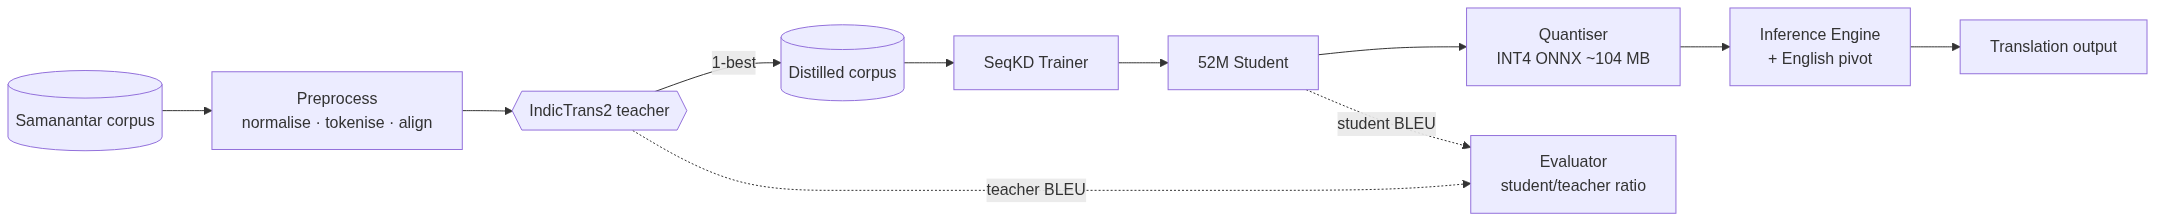
\includegraphics[width=0.96\textwidth, height=0.72\textheight, keepaspectratio]{figures/data_flow.png}
\caption{Level-1 data flow diagram --- corpus to deployed translation}
\label{fig:dfd}
\end{figure}

\subsection{Entity-Relationship Model}
\label{subsec:er}

\setu{} does not use a relational database --- an offline edge deployment should
not require one --- but its persistent artifacts have a clear relational
structure, recorded in Figure~\ref{fig:er}. Corpora are stored as JSONL,
reports as JSON, models as ONNX with an accompanying SentencePiece tokenizer,
and the language registry as YAML.

\begin{figure}[H]
\centering
\begin{tikzpicture}[node distance=13mm and 20mm]
  \node[ent, minimum width=30mm] (lang) {\textbf{Language}\\\scriptsize iso, flores, script, endonym};
  \node[ent, below=22mm of lang, minimum width=32mm] (pair) {\textbf{LanguagePair}\\\scriptsize src\_flores, tgt\_flores};
  \node[ent, left=of pair, minimum width=30mm] (sent) {\textbf{SentencePair}\\\scriptsize src\_text, tgt\_text, source};
  \node[ent, right=of pair, minimum width=32mm] (mv) {\textbf{ModelVersion}\\\scriptsize params, quant\_bits, size\_mb};
  \node[ent, below=20mm of sent, minimum width=32mm] (ev) {\textbf{EvalReport}\\\scriptsize bleu, chrf, teacher\_bleu, ratio};
  \node[ent, below=20mm of mv, minimum width=32mm] (tr) {\textbf{TranslationResult}\\\scriptsize text, latency\_ms, pivot};

  \node[dec, above=7mm of pair, text width=20mm] (has) {defines};
  \node[dec, left=6mm of pair, text width=18mm, xshift=-2mm] (cont) {contains};
  \node[dec, right=6mm of pair, text width=18mm, xshift=2mm] (trained) {trains};
  \node[dec, below=6mm of sent, text width=18mm] (scored) {scored by};
  \node[dec, below=6mm of mv, text width=18mm] (prod) {produces};

  \draw[-] (lang) -- node[lbl,right]{2} (has);
  \draw[-] (has)  -- node[lbl,right]{1} (pair);
  \draw[-] (pair) -- node[lbl,above]{N} (cont);
  \draw[-] (cont) -- node[lbl,above]{1} (sent);
  \draw[-] (pair) -- node[lbl,above]{1} (trained);
  \draw[-] (trained) -- node[lbl,above]{N} (mv);
  \draw[-] (sent) -- node[lbl,right]{N} (scored);
  \draw[-] (scored) -- node[lbl,right]{1} (ev);
  \draw[-] (mv)   -- node[lbl,right]{1} (prod);
  \draw[-] (prod) -- node[lbl,right]{N} (tr);
  \draw[-, dashed, black!55] (mv) -- node[lbl,above,pos=0.5]{evaluated by} (ev);
\end{tikzpicture}
\caption{Entity-relationship model of \setu{}'s persistent artifacts}
\label{fig:er}
\end{figure}

\subsection{Class Diagram}
\label{subsec:class}

Figure~\ref{fig:class} gives the principal classes. The design deliberately
isolates every dependency on the teacher's implementation inside a single class,
\texttt{IndicTrans2Teacher}. A unit test scans the source tree and fails the
build if any other module imports \texttt{transformers}, \texttt{torch} or
\texttt{IndicTransToolkit}. This is what allows the deployed artifact to contain
no training dependencies at all.

\begin{figure}[H]
\centering
\scalebox{0.97}{%
\begin{tikzpicture}[node distance=8mm and 10mm]
  \node[cls] (teacher) {%
    \textbf{TeacherModel} \textit{(abstract)}\clsrule + generate\_candidates(src, n)\\
    + generate\_candidates\_batch(...)\\
    + score\_candidates(cands, ref)};
  \node[cls, below=of teacher] (it2) {%
    \textbf{IndicTrans2Teacher}\clsrule -- model, -- processor\\
    \textit{sole importer of transformers/torch}};
  \node[cls, right=18mm of teacher] (dist) {%
    \textbf{SeqKDDistiller}\clsrule -- teacher, -- batch\_size, -- stats\\
    + distill(entries) $\rightarrow$ entries};
  \node[cls, below=of dist] (sft) {%
    \textbf{SFTTrainer}\clsrule -- model, -- optimizer, -- scheduler\\
    -- label\_smoothing, -- max\_grad\_norm\\
    + train(dataset)};
  \node[cls, below=of sft] (dpo) {%
    \textbf{DPOTrainer}\clsrule -- policy, -- frozen reference\\
    -- beta \quad + train(pairs)};
  \node[cls, below=of it2] (tok) {%
    \textbf{StudentTokenizer}\clsrule -- sp\_model, -- vocab\_size\\
    + encode / decode / encode\_target};
  \node[cls, below=of tok] (cfg) {%
    \textbf{ModelConfig}\clsrule language\_pair, params,\\quantization};
  \node[cls, right=18mm of sft] (eng) {%
    \textbf{InferenceEngine}\clsrule -- onnx\_engine, -- is\_stub\\
    + translate(text, src, tgt)};
  \node[cls, above=of eng] (onnx) {%
    \textbf{ONNXTranslator}\clsrule -- session, -- tokenizer\\
    + generate(ids) $\rightarrow$ ids};
  \node[cls, below=of eng] (router) {%
    \textbf{Router}\clsrule -- engine cache (per pair)\\
    + translate(...) $\rightarrow$ (result, pivot, stub)};
  \node[cls, below=of router] (res) {%
    \textbf{TranslationResult}\clsrule translated\_text, latency\_ms,\\src\_lang, tgt\_lang, pivot};

  \draw[-{Triangle[open, length=2.4mm]}] (it2) -- (teacher);
  \draw[fl] (dist) -- node[lbl,above]{uses} (teacher);
  \draw[fl] (sft)  -- node[lbl,above]{trains on} (dist);
  \draw[fl] (dpo)  -- node[lbl,left]{frozen ref} (sft);
  \draw[fl] (sft)  -- node[lbl,above]{tokenises with} (tok);
  \draw[fl] (tok)  -- (cfg);
  \draw[fl] (eng)  -- node[lbl,left]{delegates} (onnx);
  \draw[fl] (router) -- node[lbl,left]{caches} (eng);
  \draw[fl] (router) -- node[lbl,left]{returns} (res);
  \draw[fl] (eng)  -- node[lbl,above]{loads} (sft);
\end{tikzpicture}}
\caption{Class diagram --- training classes (left) are used offline by the ML Engineer; inference classes (right) ship to the device}
\label{fig:class}
\end{figure}

\section{Software Requirements Specification}
\label{sec:srs}

This section states what the system must do, independently of how it does it.

\subsection{User Requirements}
\label{subsec:userreq}

\begin{table}[H]
\centering
\caption{User requirements}
\label{tab:userreq}
\begin{tabular}{@{}p{1.4cm} p{2.6cm} p{9.8cm}@{}}
\toprule
\rowcolor{headblue}
\textbf{ID} & \textbf{User} & \textbf{Requirement} \\
\midrule
UR-1 & End user & Translate text between any two supported languages without an internet connection \\
\rowcolor{rowgrey}
UR-2 & End user & See which languages are available and which are not yet trained, before attempting a translation \\
UR-3 & End user & Receive a translation quickly enough for conversational use \\
\rowcolor{rowgrey}
UR-4 & End user & Be assured that the text typed never leaves the device \\
UR-5 & End user & Use the system from a browser, a mobile application, a command line or a programmatic API, with identical behaviour \\
\rowcolor{rowgrey}
UR-6 & ML engineer & Train a model for any language pair by changing configuration, without modifying source code \\
UR-7 & ML engineer & Resume a multi-hour training run after a disconnection without repeating completed stages \\
\rowcolor{rowgrey}
UR-8 & ML engineer & Obtain an honest quality report, including failure, rather than an optimistic one \\
UR-9 & Deployer & Install models on a fresh machine and run the system without training anything \\
\bottomrule
\end{tabular}
\end{table}

\subsection{System Requirements}
\label{subsec:sysreq}

\begin{itemize}
  \item \textbf{SR-1.} Python 3.11 or 3.12; Python 3.14 is incompatible with the
        teacher's remote modelling code.
  \item \textbf{SR-2.} \texttt{transformers} at least 4.42 and below 4.54, since
        4.54 removed the legacy tuple \texttt{past\_key\_values} cache API that
        the rotary teacher relies on.
  \item \textbf{SR-3.} PyTorch 2.6 or newer for training, paired with a matching
        \texttt{torchvision} build.
  \item \textbf{SR-4.} ONNX Runtime with the CPU execution provider for
        inference; no GPU dependency in the deployed artifact.
  \item \textbf{SR-5.} A CUDA-capable GPU with at least 16\,GB of memory for
        training a direction.
  \item \textbf{SR-6.} At least 104\,MB of free storage per translation
        direction on the target device.
  \item \textbf{SR-7.} Node.js 18 or newer to build the browser client (build
        time only; the exported application is static).
\end{itemize}

\subsection{Functional Requirements}
\label{subsec:funcreq}

\begin{longtable}{@{}p{1.4cm} p{7.8cm} p{4.6cm}@{}}
\caption{Functional requirements}
\label{tab:funcreq}\\
\toprule
\rowcolor{headblue}
\textbf{ID} & \textbf{Requirement} & \textbf{Verified by} \\
\midrule
\endfirsthead
\multicolumn{3}{c}{\textit{Table \thetable{} --- continued from previous page}}\\
\toprule
\rowcolor{headblue}
\textbf{ID} & \textbf{Requirement} & \textbf{Verified by} \\
\midrule
\endhead
\midrule
\multicolumn{3}{r}{\textit{continued on next page}}\\
\endfoot
\bottomrule
\endlastfoot

FR-1 & Translate text between supported Indian languages and English in both directions, fully offline & \S\ref{subsec:unittest}, \S\ref{sec:testreports} \\
\rowcolor{rowgrey}
FR-2 & Accept plain-text input of up to 512 tokens per request & \S\ref{subsec:unittest} \\
FR-3 & Reject a request whose source and target language are identical & UT-2 \\
\rowcolor{rowgrey}
FR-4 & Reject a request containing an unknown language code & UT-3 \\
FR-5 & Route Indic-to-Indic pairs through English when no direct model exists, and report that it did so & IT-1 to IT-3 \\
\rowcolor{rowgrey}
FR-6 & Expose \texttt{POST /translate}, \texttt{GET /languages}, \texttt{GET /models} and \texttt{GET /health} & \S\ref{sec:interface}, IT-4 \\
FR-7 & Discover every model present on disk at start-up and report its variant and size & IT-4 \\
\rowcolor{rowgrey}
FR-8 & Generate teacher one-best targets for an arbitrary corpus slice & \S\ref{subsec:mod2} \\
FR-9 & Train a student on either distilled or reference targets, selectable at run time & \S\ref{subsec:mod3} \\
\rowcolor{rowgrey}
FR-10 & Quantise a trained student to INT8 and INT4 ONNX with a per-stage benchmark & \S\ref{subsec:mod4} \\
FR-11 & Report BLEU, chrF and the student/teacher ratio per direction & \S\ref{sec:testreports} \\
\rowcolor{rowgrey}
FR-12 & Support incremental addition of a language by configuration alone & \S\ref{subsec:mod8} \\
\end{longtable}

\subsection{Non-Functional Requirements}
\label{subsec:nonfuncreq}

\begin{table}[H]
\centering
\caption{Non-functional requirements and measured outcomes}
\label{tab:nonfuncreq}
\begin{tabular}{@{}p{1.3cm} p{2.4cm} p{4.6cm} p{5.4cm}@{}}
\toprule
\rowcolor{headblue}
\textbf{ID} & \textbf{Attribute} & \textbf{Requirement} & \textbf{Measured outcome} \\
\midrule
NFR-1 & Performance & Under 500\,ms per sentence on ARM-class CPU & Mean 105--202\,ms; p90 141--541\,ms (one outlier) \\
\rowcolor{rowgrey}
NFR-2 & Size & At most 200\,MB per direction after quantisation & 103.9\,MB for every direction \\
NFR-3 & Accuracy & At least 80\,\% of teacher BLEU & 14 of 22 directions; mean ratio 0.838 \\
\rowcolor{rowgrey}
NFR-4 & Availability & Fully functional offline after initial setup & Verified with all sockets disabled \\
NFR-5 & Privacy & No user text transmitted during inference & Verified by code audit and the offline test \\
\rowcolor{rowgrey}
NFR-6 & Portability & Runs on x86-64 and ARM, Linux and Android & ONNX Runtime CPU provider on both \\
NFR-7 & Maintainability & Single shared engine behind every interface & \texttt{setu.inference.router} \\
\rowcolor{rowgrey}
NFR-8 & Testability & Automated suite covering every module & 85 tests \\
NFR-9 & Reliability & Degrade explicitly, never silently & Stub engine reports \texttt{stub:true}; scorecard reports \textsc{unverified} without evidence \\
\bottomrule
\end{tabular}
\end{table}

\subsection{Domain Requirements}
\label{subsec:domainreq}

\begin{itemize}
  \item \textbf{DR-1.} Language identification must follow the script-qualified
        FLORES convention used by IndicTrans2 (\texttt{hin\_Deva},
        \texttt{eng\_Latn}), because several scheduled languages are written in
        more than one script. Kashmiri, Manipuri and Sindhi accordingly carry
        dual-script registry entries.
  \item \textbf{DR-2.} Script normalisation must preserve zero-width joiners and
        non-joiners, which are semantically significant in Indic scripts; naive
        control-character stripping corrupts valid text.
  \item \textbf{DR-3.} Corpus cleaning must enforce a minimum fraction of
        letters in the expected script, so that mined pairs with the wrong
        language on one side are removed.
  \item \textbf{DR-4.} Evaluation must always use real human references held out
        from training, never teacher output, regardless of what the student was
        trained on. This is what makes the comparison in
        Section~\ref{sec:headtohead} fair.
  \item \textbf{DR-5.} Tokenizer language tags must be reserved for all 22
        scheduled languages from the first training run, so that token
        identifiers remain stable when languages are added later and previously
        trained models need not be re-tokenised.
  \item \textbf{DR-6.} BLEU must not be compared across languages. Agglutinative
        languages such as Malayalam and Tamil score low in absolute BLEU for
        morphological reasons; only the student/teacher ratio is comparable
        across directions.
\end{itemize}
